\subsection{Invasibilidad C-R}\label{subsec:InvCR}

En particular dado que $f_1(k_{\RC}) \to 0$ (cuando $k_{\RC} \to 0)$ y $\beta <1$ tenemos que $\chi_1 \to 0 (k_{\RC} \to 0)$, para un valor acotado de $\kappa_0$,y por lo tanto valores extremadamente peque\~nos de $k_{\RC}$ siempre ser\'an exclu\'idos de $\mathbf{Z(I_{\C\to \R})}$ si mantenemos $m_\PP$ y $k_{\CP}$ constante(un comportamiento an\'alogo se observa para $k_\CP$ peque\~nos), dicho esto al aumentar $k_{\CP}$, $\kappa_0$ y $m_P$ el m\'inimo $k_{\RC}$ disminuye, asu vez dado que el impacto de $m_P$ y $k_\CP$ esta influenciado por la dimensi\'on del espacio de b\'usqueda esta disminuci\'on es mas fuerte para ambientes $3D$.\\

Para valores fijos de $k_{\CP}, \kappa_0 ,m_P$,el valor m\'aximo de $k_{\RC}$ en $\mathbf{Z(I_{\C\to \R})}$ depender\'a del valor de $\phi$ y $Fm$. Sin embargo para los distintos $Fm$ tenemos un comportamiento cualitativo similar , debido a la similitud existente entre $f_1$ para distintos $Fm$(v\'ease anexo \ref{subsec:funcf}). Dada la similitud entre $g$ y $f_1$ por un tratamiento similar al descrito en anexos \ref{subsec:funcf} podemos observar que para $\phi$ \emph{suficientemente peque\~no} $\chi_1$ crece mon\'otonamente con respecto a $k_\RC$ por lo tanto se observa la presencia de un valor umbral $k$ tal que por encima de \'el la invasi\'on de $C$ es posible. A su vez para valores de $\phi$ \emph{suficientemente grandes} tenemos que $\chi_1$ presenta un valor m\'aximo por encima del cual decrece mon\'otonamente, es m\'as $\chi_1 \approx c k_{RC}^{h - \phi}$ para valores de $k_\RC$ elevados (donde $h$ depende de $Fm$) y por tanto estos ser\'ian exclu\'idos de $\mathbf{Z(I_{\C\to \R})}$ dado que al mantener $m_P$ y $k_\CP$ fijos cambios en $k_\RC$ simplemente indican cambios en la masa de $m_R$ podemos interpretar estos resultados de la siguiente manera, sin importar $\phi$, $m_R$ tiene que tener un tama\~no m\'inimo el cual permita a $C$ invadir, esto debido al hecho que $m_R$ influencia la capacidad de carga de $R$, y por ende la energ\'ia disponible a $C$ al momento de la invasi\'on, sin embargo valores elevados de $m_R$ son inviables para $C$ para $\phi$ \emph{suficientemente grandes} ya que en estos casos a pesar de que el sistema presenta una gran cantidad de energ\'ia disponible, debido a la baja probabilidad de captura de $R$ por parte de $C$ no se traducen en aumentos en biomasa de $C$, es decir lo importante para $C$ al momento de la invasi\'on no solamente es la energ\'ia total presente en el sistema sino que \'esta se encuentre en una \emph{forma} que pueda ser explotada por $C$.\\

Si mantenemos $\kappa_0,k_\CP$ y $k_\RP$ fijos, observamos que para que sea posible la invasi\'on de $C$, $m_P$ tiene que superar un valor dado. Dado que aumentos en $m_P$ para raz\'on de masas fijos implican aumentos en las masas de $R$ y $C$ respectivamente, esto nos dice que existe un tama\~no de $C$ y$R$ por encima del cual la invasi\'on de $C$ es posible.

La dimensi\'on del espacio de b\'usqueda afecta positivamente en la mayoria de los casos a $\chi_1$(si asociamos cambios en $\kappa_0$, y con $k_\RC > 10^{-30}$), sin embargo debido a que tambi\'en influencia positivamente a $h_R$ su impacto total sobre la invasibilidad puede ser negativo para valores elevados de $k_\RC$(i.e., cuando el m\'inimo $k_\RC$ necesario para la invasi\'on es elevado, como se da para $k_\CP$ y $m_P$ peque\~nos), siendo m\'as precisos siempre que $\frac{q_{0,1}}{\chi_1} >1$ en ambientes $2D$ tenemos que el impacto es positivo, pero para $\frac{q_{0,1}}{\chi_1} < 1$ el impacto es negativo si $ (\frac{q_{0,1}}{\chi_1})_{3D}^\frac{1 + h_{2D} - 2 \beta}{1 + h_{3D} - 2 \beta} >  (\frac{q_{0,1}}{\chi_1})_{2D} $.\\ La figura \ref{fig:Z(IC2)} muestra las distintas zonas de invasibilidad que se forman, para las distintas combinaciones de par\'ametros explorados.


\begin{figure}
  \centering
  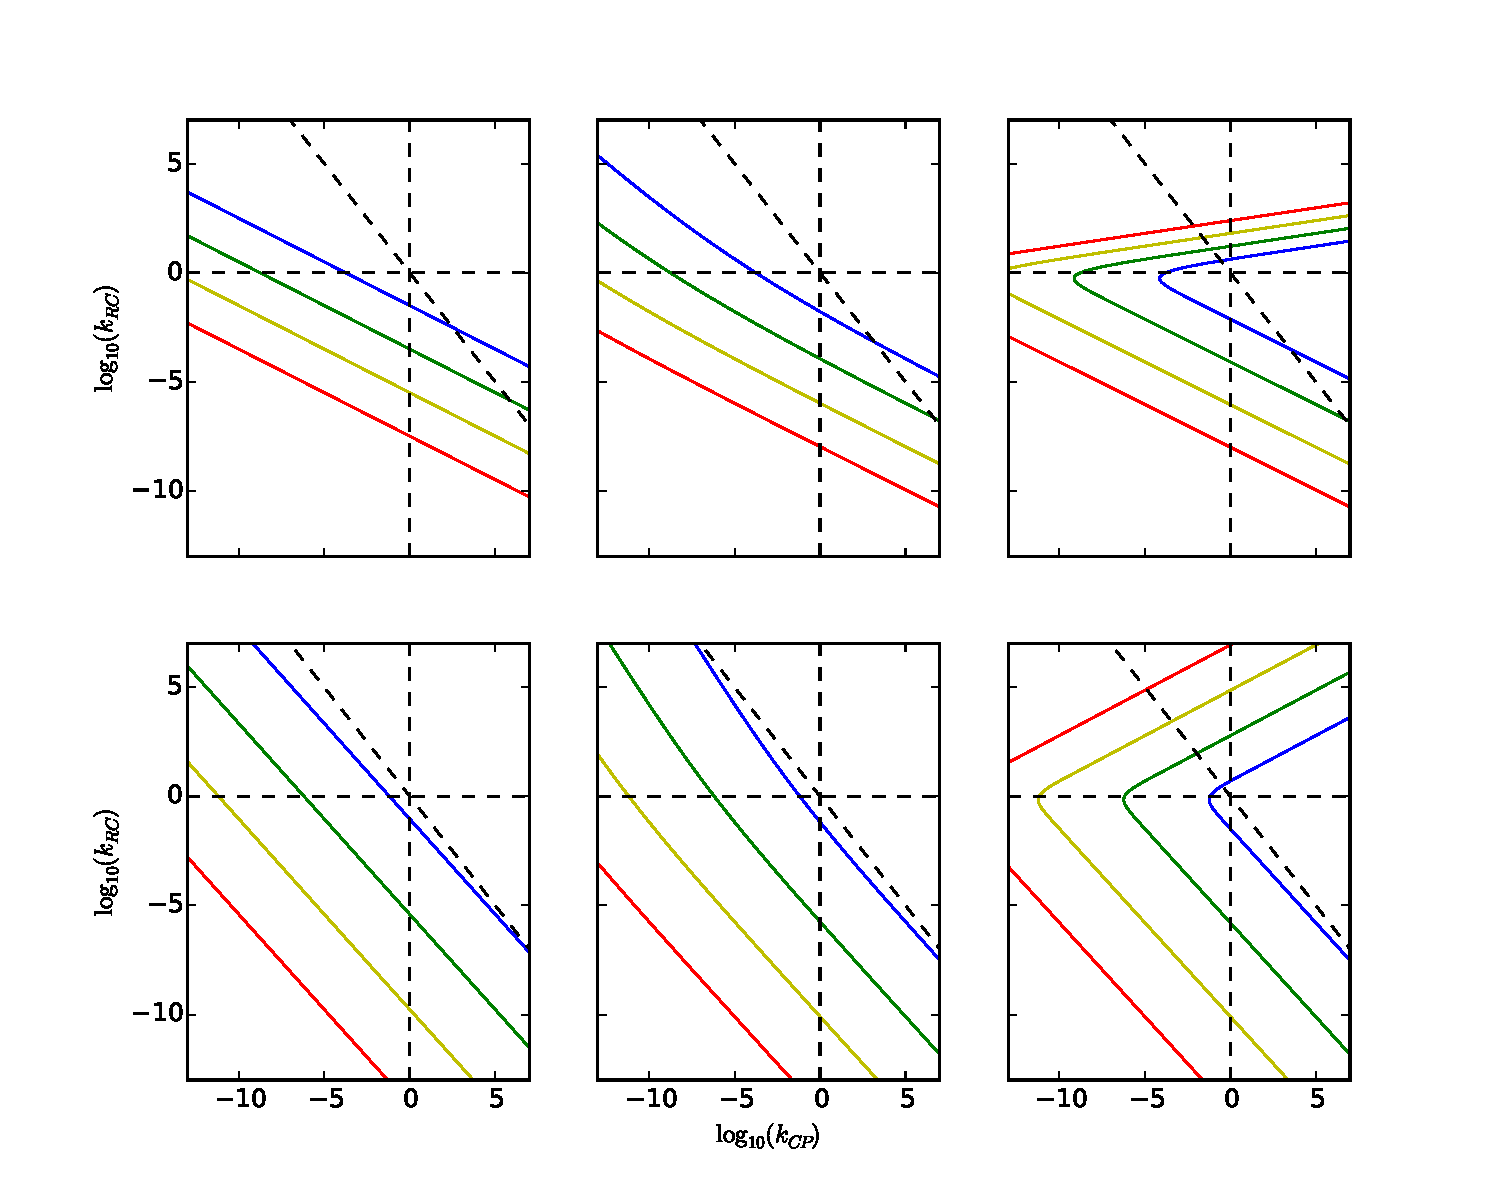
\includegraphics[width = 0.99\textwidth]{./Plots/Z(IC2)AcGrGr.pdf}
  \caption[Env $Z(IC2)$]{\emph{Envolturas de Invasibilidad} para el caso de el depredador intermedio $C$ como invasor frente a una comunidad receptora formada por $R$. La fila superior es para espacios de b\'usqueda bidimensionales y la inferior tridimensionales, las columnas de izquierda a derecha aumentan el valor de $\phi$, siendo $0.02,0.2$ y $2$ respectivamente.Las diferentes lineas implican distintas masas de depredador $m_P$ :({\hwplotR}) $10^5 kg$,  ({\hwplotY}) $1kg$, ({\hwplotG}) $10^{-5}kg$ y ({\hwplotB}) para $10^{-10}kg$. ({\hwplotK}) separa las zonas donde $K_{RC},K_{CP},k_{RP}$ son mayores o menores que 1 respectivamente. $k_0 = 0.1$ y $k_0 = 30$ para el caso $2D$ y $3D$ respectivamente, los valores de los otros par\'ametros son los descritos en el anexo \ref{subsec:params}}
  \label{fig:Z(IC2)}
\end{figure}
